\section{Threshold voltages ($V_T$)}

The threshold voltage dependence on the doping density is illustrated with \autoref{img:overview_doping_threshold} for both n-type and p-type MOSFETs with an aluminum gate metal.
\begin{figure}[H]
	\centering
	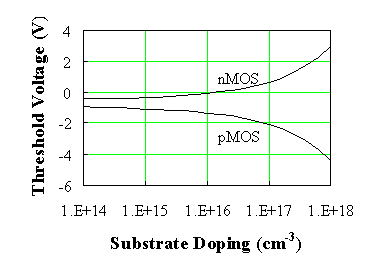
\includegraphics[scale=0.5]{doping_thresholds_overview.png}
	\caption{Threshold voltage of n-type (upper curve) and p-type (lower curve) MOSFETs versus substrate doping density.}
	\label{img:overview_doping_threshold}
\end{figure}
\begin{mdframed}[linewidth=2pt,linecolor=red]
We can directly switch $\frac{J}{C}$ with Volts because these two units are equal!\footnote{\url{https://en.wikipedia.org/wiki/Volt}}
Also $V_{th}$ will be treated as a constant for any further calculations within this document.\\

The same goes for the $eV$ to $V$ conversion, wherever we have work functions to potentials because (e.g. $\Phi_M$ for Aluminum):
$4.1 eV \approx 6.56892414528 10^{-19}J$ \\
$\Phi_M=\frac{E_M}{q}=\frac{4.1 eV}{q}=\frac{6.56892414528 10^{-19} J}{q} = \frac{6.56892414528 10^{-19} J}{1.602176634 10^{-19} C} \approx 4.099999966220953 \frac{J}{C} = \underline{4.1V}$ \\
\end{mdframed}

The formula for calculating the threshold voltage of a MOS device is the following:
\begin{equation}
V_T = V_{t-mos} + V_{FB}
\end{equation}
where $V_{t-mos}$ is the threshold voltage of an ideal MOS capacitor, $V_{FB}$ is the flat-band voltage and $V_{t-mos}$ is the threshold.
The MOS threshold voltage, $V_{t-mos}$ is calculated by considering the MOS capacitor structure that form the gate of the MOS transistor.

The ideal threshold voltage may be expressed as:
\begin{equation}
V_{t-mos}=2 \phi_F + \frac{Q_b}{C_{ox}}
\end{equation}
\begin{equation}
Q_b
=
\sqrt{2 \epsilon_{Si} \cdot q \cdot N  \cdot  ( \left| 2 \phi_F \right| + V_{SB}) }
\end{equation}
where $C_{ox}$ is the oxide capacitance and $Q_b$ which is called the bulk charge term.\\

The bulk potential is given for P substrate ($V_{Tp}$)
\begin{equation}
\phi_{Fp}
=
V_{th} \cdot ln\left(\frac{N_p}{N_i}\right)
\end{equation}
and N substrate  ($V_{Tn}$), respectively:
\begin{equation}
\phi_{Fn}
=
V_{th} \cdot ln\left(\frac{N_i}{N_n}\right)
\end{equation}

$V_{th}$ is the thermal voltage.\footnote{\url{https://en.wikipedia.org/wiki/Boltzmann_constant\#Role_in_semiconductor_physics:_the_thermal_voltage}}
\begin{equation}
V_{th} = \frac{k T}{q} \approx 0.026 \frac{J}{C} = 0.026 V = 26mV
\end{equation}

Since we connect bulk and source $V_{SB}=0$ we can simplify the equation to become
\begin{equation}
Q_b
=
\sqrt{2\cdot\epsilon_{Si}\cdot q\cdot N \cdot  ( \left| 2 \cdot \phi_F \right|) }
\end{equation}
\begin{equation}
Q_b
=
2\cdot\sqrt{\epsilon_{Si}\cdot q\cdot N \cdot \left| \phi_F \right| }
\end{equation}


$V_{FB}$, is given by:
\begin{equation}
V_{FB}
=
\phi_{MS}-\frac{Q_{SS}}{C_{ox}}-\frac{1}{C_{ox}}\int_{0}^{t_{ox}}\frac{x}{x_{ox}}\rho(x) dx
\end{equation}

Because we're not yet dealing with non-volatile memory devices which contain an oxide surface state charge we can just $\rho(x)=0$.
$Q_{SS}$ is a value which has to be measured.

\begin{equation}
V_{FB}
=
\phi_{MS} - \frac{Q_{SS}}{C_{ox}}
\end{equation}

This brings us to a general equation for the threshold voltage $V_T$:
\begin{equation}
V_T = 2 \phi_F + \frac{2\cdot\sqrt{\epsilon_{Si}\cdot q\cdot N \cdot \left| \phi_F \right| }}{C_{ox}} + \phi_{MS} - \frac{Q_{SS}}{C_{ox}}
\end{equation}

With the variables and constants being the following for both sub chapters:
\begin{itemize}
\item $N_i$ is the carrier concentration in intrinsic (undoped) silicon. $N_i$ is equal to $1.45 \times 10^{10} cm^{-3} = 1.45 \times 10^{16} m^{-3}$ at 300\degree K
\item $Q_{SS}$ depends on the process and is measured. Usually it's between $10^{9}\frac{1}{cm^2}$ and $10^{10}\frac{1}{cm^2}$ ergo  $Q_{SS} = q \cdot 10^{10}\frac{1}{cm^2} = 1.6 \cdot 10^{-5}\frac{C}{m^2}$
\item $E_M = q\cdot\phi_M = 4.1 eV$ is the "work function" of our metal at the gate (Aluminum)
\item $E_g=E_g(300) [eV]$ \\
$E_g(T) = E_g(0) - \frac{\alpha T^2}{T+\beta} = 1.166 - 4.73 \cdot 10^{-4} \cdot \frac{T^2}{T+636} [eV]$ is the band gap energy of silicon at a given temperature\footnote{\url{https://ecee.colorado.edu/~bart/book/eband5.htm}} for which the parameters can be taken from \autoref{band_gap_parameters}
\begin{table}[H]
\centering
\begin{tabular}{|c|c|c|c|}
\hline
{} &
\textbf{Germanium} &
\textbf{Silicon} &
\textbf{GaAs} \\
\hline
$Eg(0) [eV]$ &
0.7437 &
1.166 &
1.519 \\
\hline
$\alpha [eV/K]$ &
4.77 x 10-4 &
4.73 x 10-4 &
5.41 x 10-4 \\
\hline
$\beta [K]$ &
235 &
636 &
204 \\
\hline
\end{tabular}
\caption{Band cap energy parameters}
\label{band_gap_parameters}
\end{table}
\item $C_{ox} \left[\frac{F}{m^2}\right]$ is the capacity of the gate oxide
\item $\epsilon_0 = 8.85 \cdot 10^{-14} \frac{F}{cm}.= 8.85 \cdot 10^{-12} \frac{F}{m} $ is the electric permittivity in vacuum
\item $\epsilon_{Si} =11.68 \cdot \epsilon_0$ is the relative permittivity of silicon
\item $\epsilon_{ox} = 3.9 \cdot \epsilon_0$ is the relative permittivity of silicon oxide
\item $t_{ox} [cm]$ is the thickness of the oxide layer in cm
\item $E_{ef} = q \cdot \chi = 4.05 eV$ is the electron affinity of a silicon crystal surface\footnote{\url{https://en.wikipedia.org/wiki/Electron_affinity}}
\item $q=1.602 \cdot 10^{-19} C$ is the elementary charge
\item $k=1.38064852\cdot 10^{-23}  \frac{J}{K}$ is the Boltzmann constant
\item $T= 300 K$ the temperature, which we assume to be the room temperature for simplicity further on in this document as well.
\end{itemize}